\begin{frame}
    \frametitle{Cơ sở}
    Cho hai hệ cơ sở:
               \begin{itemize}
                  \item \((\mathbf{e}_1 ,\mathbf{e}_2)\) 
                \item \((\mathbf{e}_3 ,\mathbf{e}_4)\) 
                \end{itemize}
                \(\implies \mathbf{v}=\alpha\mathbf{e}_1 +\beta\mathbf{e}_2 =\gamma\mathbf{e}_3 +\sigma\mathbf{e}_{4}.\)
\end{frame}
\begin{frame}
    \frametitle{Cơ sở}
    \begin{columns}
        \begin{column}{0.45\textwidth}
            Cho hai hệ cơ sở:
               \begin{itemize}
                  \item \((\mathbf{e}_1 ,\mathbf{e}_2)\) 
                \item \((\mathbf{e}_3 ,\mathbf{e}_4)\) 
                \end{itemize}
                \(\implies \mathbf{v}=\alpha\mathbf{e}_1 +\beta\mathbf{e}_2 =\gamma\mathbf{e}_3 +\sigma\mathbf{e}_{4}.\)

                Giả sử: 
                \begin{itemize}
                \item \(\mathbf{e}_3 =2\mathbf{e}_1 -3\mathbf{e}_2 ,~\mathbf{e}_4 =\mathbf{e}_1 +2\mathbf{e}_2\),
                \item \(\alpha=5, \beta =3\).
                \end{itemize}
                \(\implies \mathbf{v}=\mathbf{e}_3 +3\mathbf{e}_4\).
        \end{column}
        \begin{column}{0.55\textwidth}
            Nếu \(\mathbf{e}_1 ,\mathbf{e}_2\) trực chuẩn:
            \begin{figure}[htps]
                \centering
                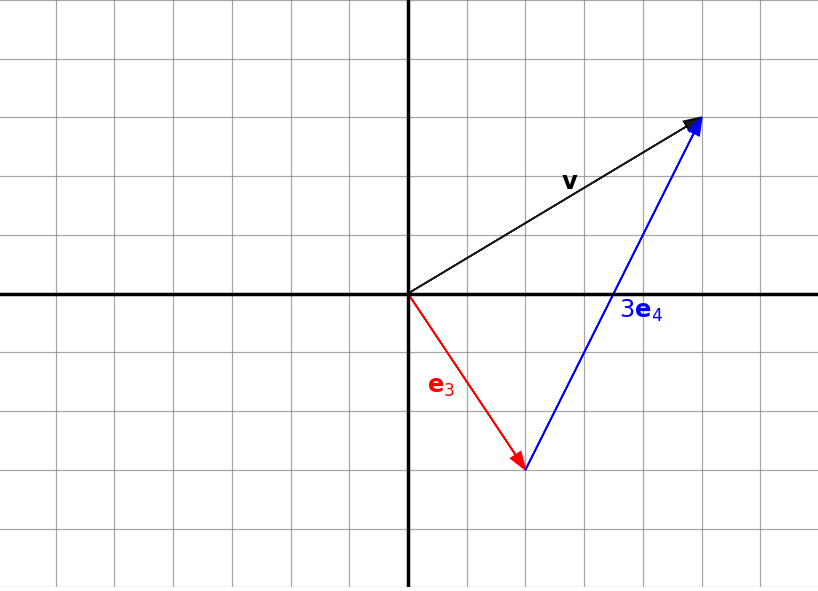
\includegraphics[width=7cm, height=5.5cm]{Slides/Figure/e3e4.png}
            \end{figure}
        \end{column}
    \end{columns}
\end{frame}
\begin{frame}
    \frametitle{Cơ sở}
    Nếu thay vì \((\mathbf{e}_3 ,\mathbf{e}_4)\), ta chọn (\(\mathbf{e}_3 ,2\mathbf{e}_3\)) thì sao?
\end{frame}
\begin{frame}
    \frametitle{Cơ sở}
    Nếu thay vì \((\mathbf{e}_3 ,\mathbf{e}_4)\), ta chọn (\(\mathbf{e}_3 ,2\mathbf{e}_3\)) thì sao?
    \begin{figure}[H]
        \centering
        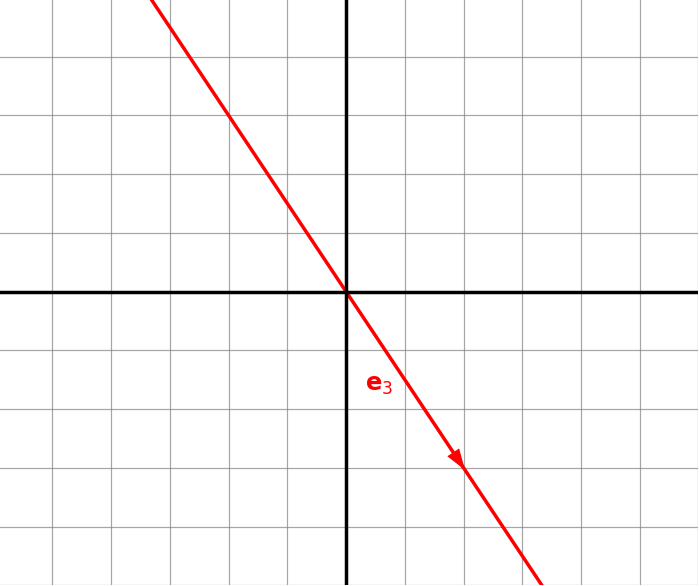
\includegraphics[width=7cm, height=6cm]{Slides/Figure/avectoronaline.png}
    \end{figure}
\end{frame}
\begin{frame}
    \frametitle{Định nghĩa}
    \begin{tcolorbox}[colback=blue!10!, colframe=blue!50!black, title=Bao tuyến tính]
        Nếu \(S=\{\mathbf{u}_{1}, \mathbf{u}_{2},\dots,  \mathbf{u}_{n}\}\) là một tập hợp \(n\) vector trong không gian, thì tập hợp tất cả các tổ hợp tuyến tính của chúng được gọi là bao tuyến tính của \(\mathbf{u}_{1}, \mathbf{u}_{2},\dots \mathbf{u}_{n}\), và được kí hiệu là span(\(S\)).
       \vspace{8pt}

        Nếu span(S) chứa toàn bộ vector trong không gian, vậy ta gọi S là một hệ sinh cho không gian.
    \end{tcolorbox}
\end{frame}
\begin{frame}
\frametitle{Định nghĩa}
    \begin{tcolorbox}[colback=blue!10!, colframe=blue!50!black, title=Độc lập tuyến tính]
        Một tập hợp các vector được gọi là \emph{độc lập tuyến tính} với nhau nếu tổ hợp tuyến tính của chúng không bao giờ bằng \(\mathbf{0}\) trừ khi \textbf{tất cả} các hệ số vô hướng đều bằng \(0\).
    \end{tcolorbox}
\end{frame}
\begin{frame}
\frametitle{Định nghĩa}
    \begin{tcolorbox}[colback=blue!10!, colframe=blue!50!black, title=Hệ cơ sở]
        Một cơ sở của không gian là một tập hợp các vector trong không gian sao cho 
    \begin{itemize}
        \item tạo thành hệ sinh cho không gian, và
        \item độc lập tuyến tính.
    \end{itemize}
    \end{tcolorbox}
\end{frame}
\begin{frame}
    \frametitle{Ví dụ}
    \begin{columns}
        \begin{column}{0.5\textwidth}
        Hệ sinh của mặt phẳng đã được đề cập:
        \begin{itemize}
            \item \(S_1=\{\mathbf{e}_1 ,\mathbf{e}_2\}\),
            \item \(S_2 =\{\mathbf{e}_3 ,\mathbf{e}_4\}\),
            \item \(S_3 =\{\mathbf{e}_3 ,\mathbf{e}_4 ,2\mathbf{e}_3\}\).
        \end{itemize}
        \end{column}
        \begin{column}{0.5\textwidth}
            Hệ sinh của đường thẳng chứa \(\mathbf{e}_3\):
            \begin{itemize}
                \item \(S_1 =\{\mathbf{e}_3\}\),
                \item \(S_2 =\{\mathbf{e}_3 ,2\mathbf{e}_3\}\),
                \item \(S_2 =\{\mathbf{e}_3 ,2\mathbf{e}_3 ,\mathbf{0}\}\).
            \end{itemize}
        \end{column}
        \end{columns}
    \vspace{10pt}

    \begin{columns}
        \begin{column}{0.5\textwidth}
            Nhưng,
            \begin{itemize}
                \item (\(\mathbf{e}_3 ,\mathbf{e}_4 ,2\mathbf{e}_3\))
            \end{itemize}
            không phải là một hệ cơ sở.
        \end{column}
        \begin{column}{0.5\textwidth}
            Nhưng,
            \begin{itemize}
                \item (\(\mathbf{e}_3 ,2\mathbf{e}_3\)), và
                \item (\(\mathbf{e}_3 ,\mathbf{0}\))
            \end{itemize}
            không phải là một hệ cơ sở.
        \end{column}
    \end{columns}
\end{frame}
\begin{frame}
    \frametitle{Ví dụ}
    Vì:
    \begin{itemize}
         \item   \(-2\mathbf{e}_{3}+1(2\mathbf{e}_{3})+0\mathbf{e}_{4}=\mathbf{0}\),
           \item \(-2\mathbf{e}_{3}+1(2\mathbf{e}_{3})=\mathbf{0}\),
        \item    \(0\mathbf{e}_3 +100(\mathbf{0})=\mathbf{0}\).
    \end{itemize}
\end{frame}
\begin{frame}
    \frametitle{Không gian vector}
    Có một sự mập mờ khi sử dụng cụm từ "không gian" trong các phần trước!
\end{frame}
\begin{frame}
    \frametitle{Không gian vector}
    Một không gian vector là một tập hợp mà các phần tử trong đó thoả mãn:
    \begin{enumerate}
        \item Với mọi \(\mathbf{v}, \mathbf{w}\in V , \mathbf{v}+\mathbf{w}\in V\).
        \item Với mọi \(\mathbf{v}\in V, \alpha\in \mathbb{R}, \alpha\mathbf{v}\in V\).
        \item \(\mathbf{v}+\mathbf{w}=\mathbf{w}+\mathbf{v}\).
        \item   \(\mathbf{u}+(\mathbf{v}+\mathbf{w})=(\mathbf{u}+\mathbf{v})+\mathbf{w}\).
        \item Tồn tại một vector \(\mathbf{0}\) sao cho \(\mathbf{v}+\mathbf{0}=\mathbf{v}\).
        \item Với mọi vector \(\mathbf{v}\), tồn tại một vector \(\mathbf{v}'\) sao cho \(\mathbf{v}+\mathbf{v}'=\mathbf{0}\).
        \item \(1\mathbf{v}=\mathbf{v}\).
        \item \(\alpha(\beta\mathbf{v})=(\alpha\beta)\mathbf{v}\).
        \item \(\alpha(\mathbf{v}+\mathbf{w})=\alpha\mathbf{v}+\alpha\mathbf{w}\).
        \item \((\alpha+\beta)\mathbf{v}=\alpha\mathbf{v}+\beta\mathbf{v}\). 
    \end{enumerate}
\end{frame}
\begin{frame}
    \frametitle{Ví dụ 1}
    Tập hợp số thực: \(\mathbb{R}^1\)
    \begin{figure}[H]
        \centering
        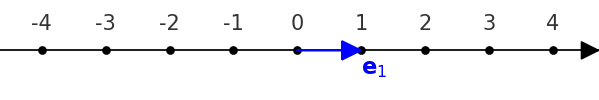
\includegraphics[width=12cm, height=2cm]{Slides/Figure/1Dvectorspace.png}
    \end{figure}
    Vector: \(-1.9, 5, 2,100, -\pi, e,\dots\)
\end{frame}
\begin{frame}
    \frametitle{Ví dụ 2}
    Mặt phẳng toạ độ: \(\mathbb{R}^2\)
    \begin{figure}[H]
        \centering
        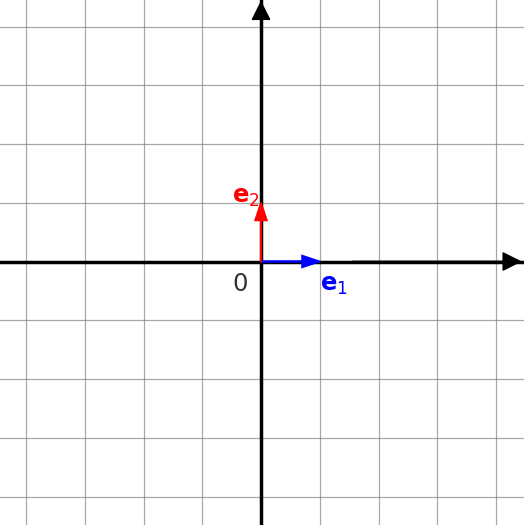
\includegraphics[width=6cm, height=4.5cm]{Slides/Figure/2Dvectorspace.png}
    \end{figure}
    Vector: \((1.23;2),(\pi, e),(-111,-\pi),\dots\)
\end{frame}
\begin{frame}
    \frametitle{Ví dụ 3}
    Không gian hình học: \(\mathbb{R}^3\)
    \begin{figure}[H]
        \centering
        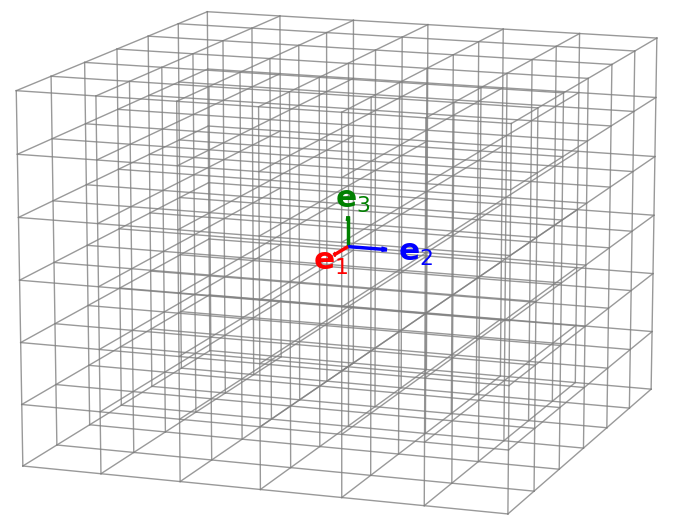
\includegraphics[width=6cm, height=4.5cm]{Slides/Figure/3Dvectorspace.png}
    \end{figure}
    Vector: \((1;3;4),(100,0,0),\dots\)
\end{frame}
\begin{frame}
    \frametitle{Chiều}
    \begin{tcolorbox}[colback=blue!10!, colframe=blue!50!black, title=Chiều của không gian vector]
        Chiều của một không gian là số lượng vector trong hệ cơ sở của không gian đó.
    \end{tcolorbox}
    
\end{frame}
\begin{frame}
    \frametitle{Chiều}
    \begin{tcolorbox}[colback=blue!10!, colframe=blue!50!black, title=Chiều của không gian vector]
        Chiều của một không gian là số lượng vector trong hệ cơ sở của không gian đó.
    \end{tcolorbox}
    \(\mathbb{R}, \mathbb{R}^2 ,\mathbb{R}^3\) đã được đề cập. Vậy \(\mathbb{R}^4, \mathbb{R}^5 ,\cdots\) thì sao?
\end{frame}
\begin{frame}
    \frametitle{Chiều}
    Vector trong   \(\mathbb{R}^4\): Mảng số có 4 thành phần.
 
    Vector trong \(\mathbb{R}^5\): Mảng số có 5 thành phần.

    \dots

    Vector trong \(\mathbb{R}^{100}\): Mảng số có 100 thành phần.
    
    Vector trong \(\mathbb{R}^{\text{n}}\): Mảng số có n thành phần!
    \begin{figure}
        \centering
        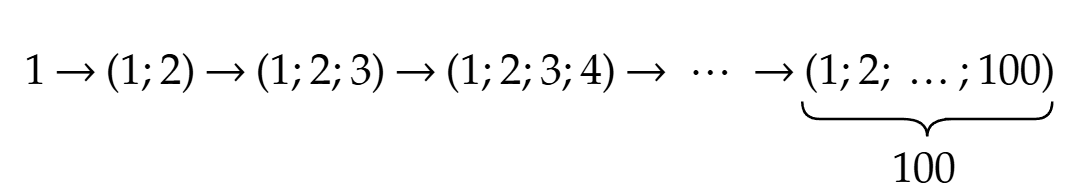
\includegraphics[width=12cm, height=2cm]{Slides/Figure/1to100.png}
    \end{figure}
\end{frame}
\begin{frame}
    \frametitle{Mũi tên hay mảng số?}
    Từ \(\mathbb{R}^4\) trở đi, không còn mũi tên nào cả.
    \begin{figure}
        \centering
        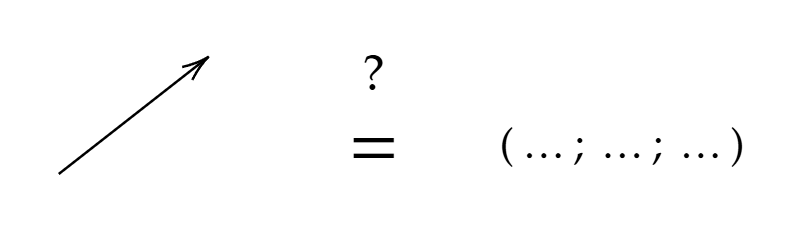
\includegraphics[width=12cm, height=3cm]{Slides/Figure/arroworarray.png}
    \end{figure}
\end{frame}
\begin{frame}
    \frametitle{Vector?}
    \begin{itemize}
        \item \(\mathbb{C}^n : (1+2i; 0.76-100i; i; e+\pi i;\dots)\).
    \end{itemize}
\end{frame}
\begin{frame}
    \frametitle{Vector?}
    \begin{itemize}
        \item \(\mathbb{C}^n : (1+2i; 0.76-100i; i; e+\pi i;\dots)\).
        \item \(f(x)=1+2x^2 -3x^3 +42x^4\).
        \item \(g(x)=\sin x\).
        \item \(\cdots\)
    \end{itemize}
\end{frame}
\begin{frame}
    \frametitle{Quay trở lại với các vector thực}
    \begin{figure}[H]
    \centering
    \begin{subfigure}[t]{0.4\textwidth}
        \centering
        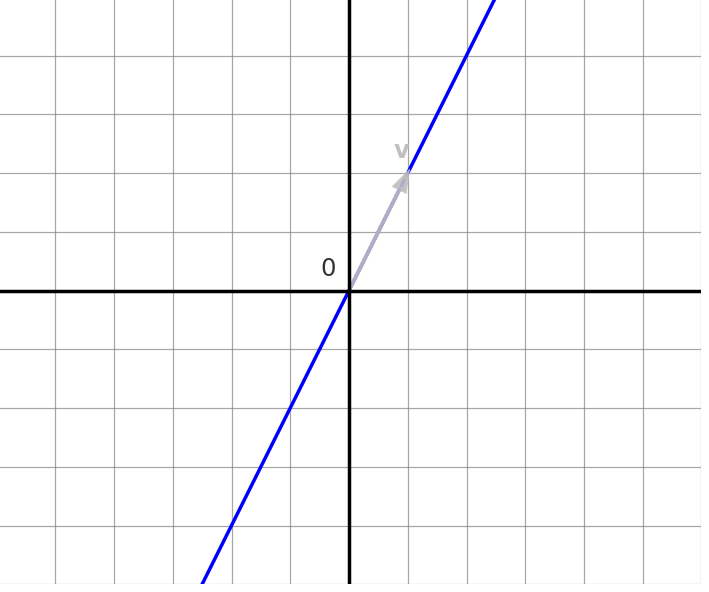
\includegraphics[width=5cm, height=5cm]{Slides/Figure/lineonplane.png}
        \caption{Đường thẳng (đi qua gốc toạ độ) trên mặt phẳng}
    \end{subfigure}
    \hfill
    \begin{subfigure}[t]{0.4\textwidth}
        \centering
        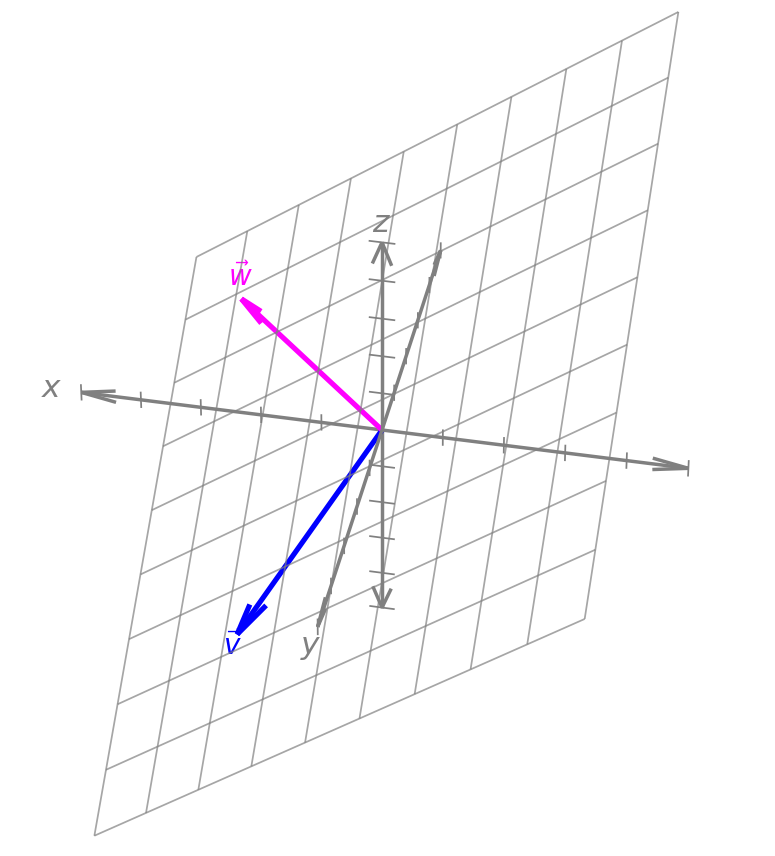
\includegraphics[width=5cm, height=5cm]{Slides/Figure/planeinspace.png}
        \caption{Mặt phẳng (đi qua gốc toạ độ) trong không gian}
    \end{subfigure}
\end{figure}
\end{frame}
\begin{frame}
    \frametitle{Không gian con}
    \begin{tcolorbox}[colback=blue!10!, colframe=blue!50!black, title=Không gian con]
        Một không gian con \(S\) trong một không gian vector \(V\) là một tập hợp các vector trong \(V\) sao cho chúng thoả mãn 10 tiên đề của vector.
    \end{tcolorbox}
    \begin{tcolorbox}[colback=blue!10!, colframe=blue!50!black, title=Cơ sở của không gian con]
        Một cơ sở cho một không gian con \(S\) của \(\mathbb{R}^n\) là một tập hợp các vector trong \(S\) sao cho 
    \begin{enumerate}
        \item tạo thành \(S\), và
        \item là độc lập tuyến tính.
    \end{enumerate}
    \end{tcolorbox}
\end{frame}
\begin{frame}
    \frametitle{Thêm ví dụ}
    Một đường thẳng đi qua gốc toạ độ trên một mặt phẳng trong không gian:
    \begin{figure}[H]
        \centering
        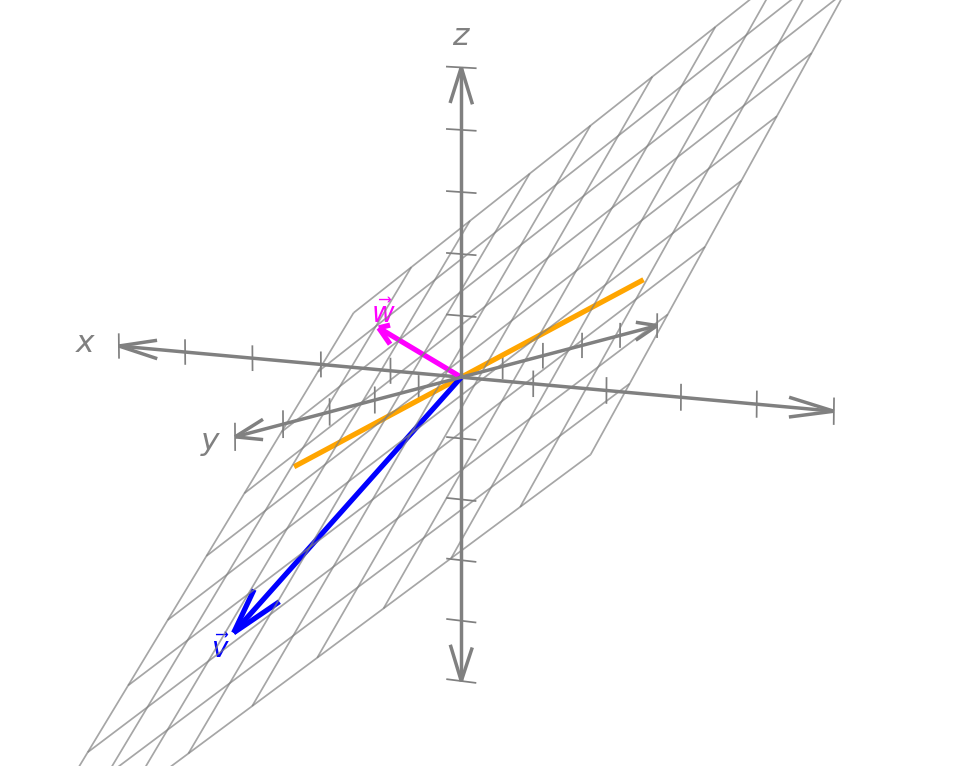
\includegraphics[width=7cm, height=5cm]{Slides/Figure/lineonplaneinspace.png}
    \end{figure}
\end{frame}